\section{Algorithm 1}
The first algorithmic approach to find the boundary-defining Hamiltonian cycle of a square lattice graph is strongly related to the proof of Theorem~\ref{FourCornerLemma}. By assuming that the westernmost vertex of the northernmost vertices always has exactly two edges rightward and downward.
\\$directions$ = $(north,east,south,west)$ correspond to $(0,1,2,3)$.
\\$Normal(d) = d+1 \pmod{4}$
\\$TileAt(x,y) =$ true if there is a tile at position x,y and false if otherwise.
\\$ApplyDirectionX(x, d) =$ if direction is horizontal, that is $d \pmod{2} = 1$, then offset x by 1 accordingly
\\Same applies for $ApplyDirectionY(y,d)$ but for vertical directions of $d \pmod{2} = 0$.
\begin{enumerate}[\bf 1.]
\item Let $G_{x,y}$ be the direction to which the tile at $(x,y)$ points to. Set all $G_{x,y}=-1$ for $x,y \in \mathbb{Z}$
\item Set $x\gets x_0, y\gets y_0$, of the coordinates $x_0,y_0$ of the westernmost vertex of the northernmost vertices of graph $G$. $currentDirection\gets 0$
\item \label{loopBegin} Set $direction \gets Normal(currentDirection) \pmod{4}$
\item \label{CoordinateSetting} $x'$ \gets ApplyDirectionX($x$, $direction$), $y'$ \gets ApplyDirectionY($y$, $direction$)
\item if not TileAt($x'$,$y'$), go to step $\ref{loopUpdate}$
\item Set $G_{x,y} = direction$, $x \gets x', y \gets y'$, $currentDirection \gets direction$.
\item if $x=x_0$ and $y=y_0$, stop, else go to step $\ref{loopBegin}$.
\item \label{loopUpdate} $direction \gets direction+1 \pmod{4}$
\item if $direction = lastDirection$, stop, else go to step ~\ref{CoordinateSetting}.
\end{enumerate}
\begin{figure}[H]
\centering
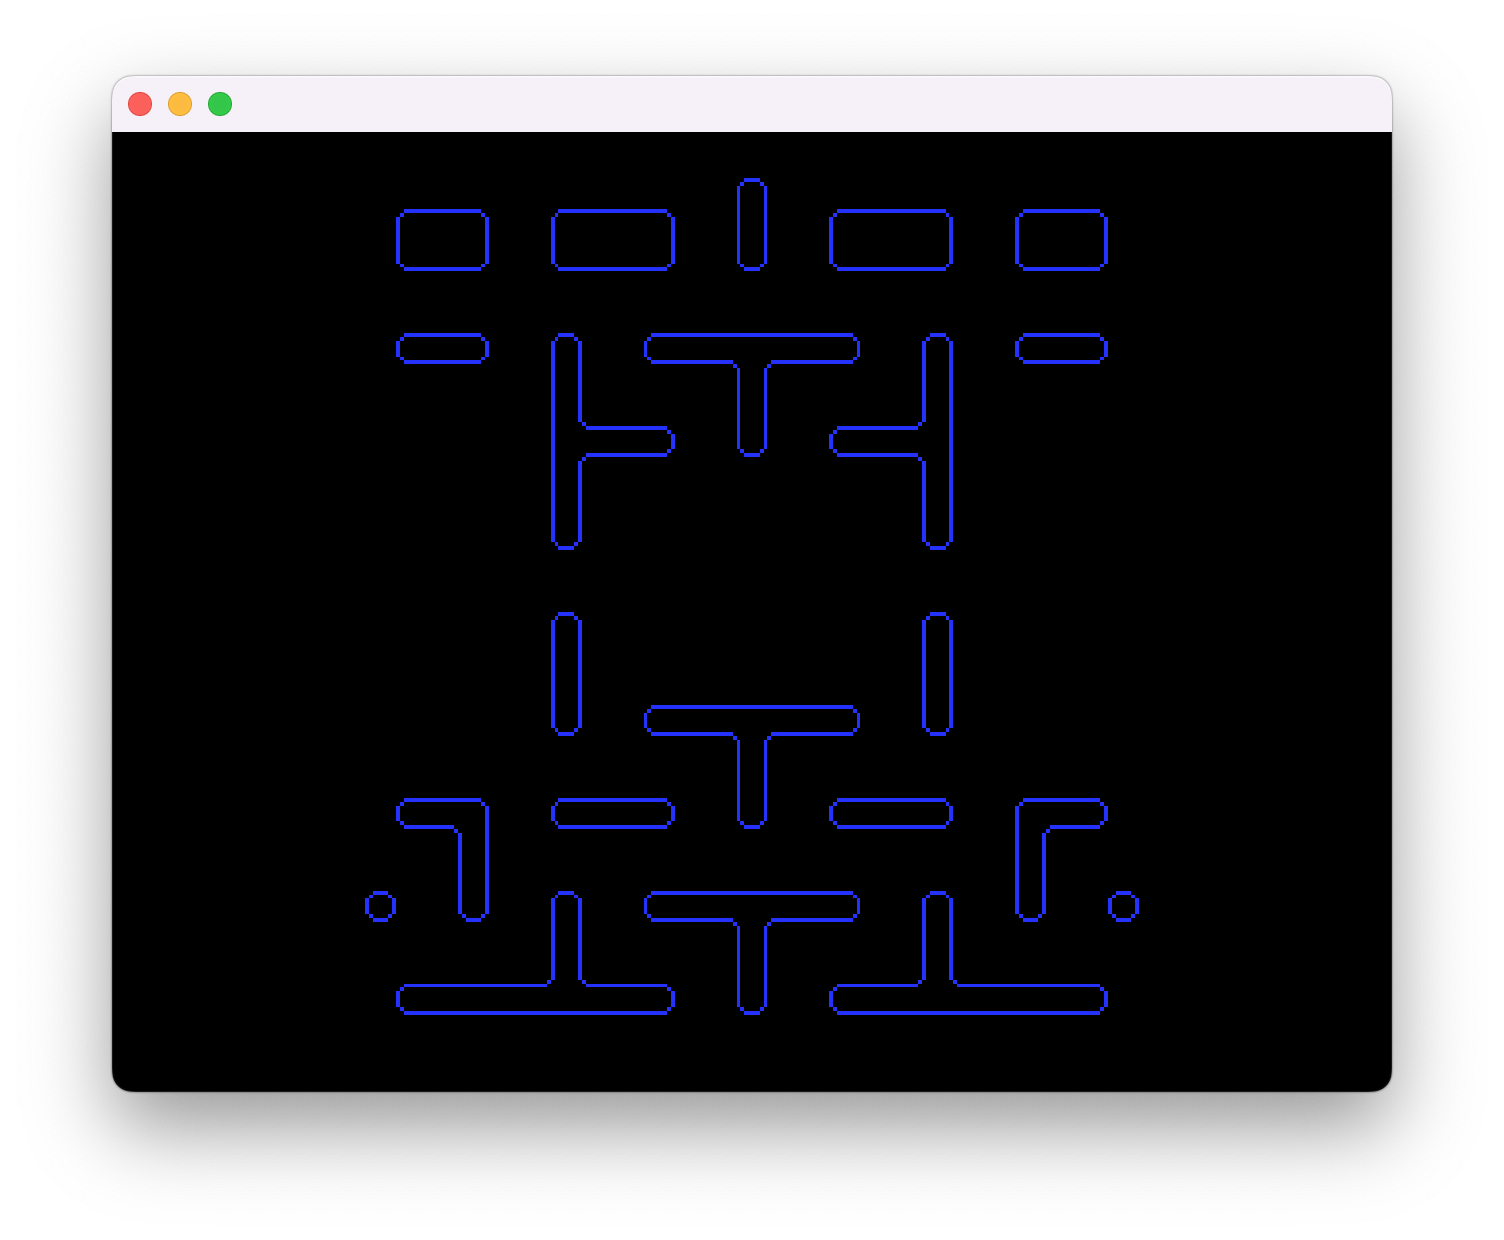
\includegraphics[width=0.8\linewidth]{Image-8.png}
\caption {Output of first algorithm\autocite{myself}}\label{FirstOutput}
\end{figure}